\section{Cloud Connectivity \& IoT}

\subsection{End-to-End Pipeline Sequence}

Figure~\ref{fig:diag-sequence} shows the complete message sequence for a single 5-second publish cycle, from CAN frame reception on the ESP32 through to dashboard rendering in the browser.

\begin{figure}[H]
    \centering
    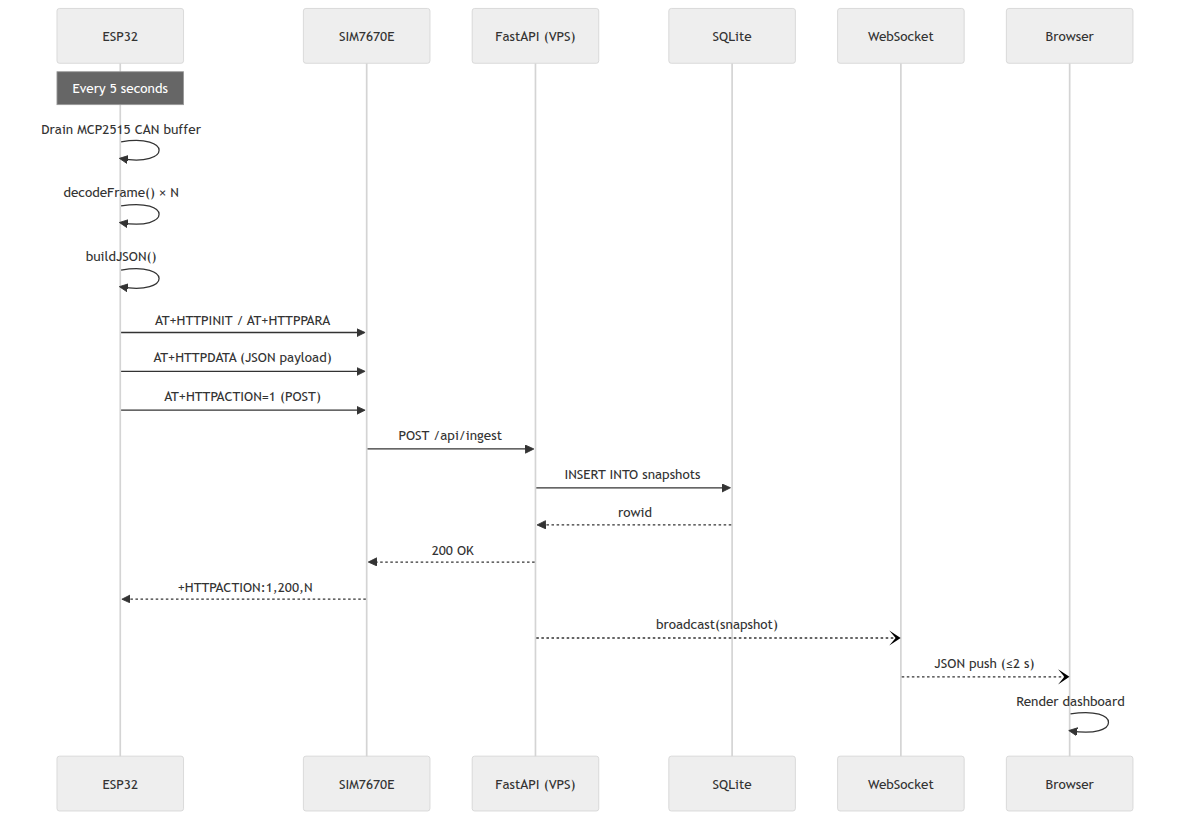
\includegraphics[width=\textwidth]{images/diag-sequence.png}
    \caption{End-to-end cloud telemetry sequence diagram: ESP32 CAN drain and JSON build, SIM800L AT command exchange, FastAPI ingest and SQLite write, WebSocket broadcast, and browser render --- one complete cycle every 5 seconds.}\label{fig:diag-sequence}
\end{figure}

This section describes the complete cloud telemetry pipeline designed and implemented for the Bako OBD ISS platform~\cite{evmonitoring}. The pipeline carries live battery data from the vehicle's CAN bus to a remote web dashboard through a sequence of embedded, network, server, and browser components. The architecture was designed to be hardware-independent: the same dashboard and backend serve both a direct USB serial connection (for lab use) and a cellular GPRS connection from the field.

% ─────────────────────────────────────────────────────────────────────────────
\subsection{Telematics \& Data Acquisition}

Telematics in this project refers to the capture, local decoding, and wireless transmission of battery state data from the moving vehicle to a remote server.

\subsubsection{On-Vehicle Data Acquisition}

Data acquisition begins at the O'CELL IFS60.8-500-F-E3 BMS, which continuously transmits CAN frames on a 250 kbps SAE J1939 bus. The ESP32 microcontroller, equipped with an MCP2515 CAN transceiver, receives all frames on this bus and decodes them in real time using the firmware described in Section~\ref{sec:bms-firmware}.

The BMS transmits at two rates. High-priority operational frames (0x18FF28F4 and 0x18FE28F4) arrive every 100 ms and carry pack voltage, current, SOC, and fault status. Lower-priority frames carrying cell-level voltages and temperatures arrive every 500 ms. At 250 kbps the bus is far from saturated; the five BMS frame types together occupy less than 2\% of available bandwidth.

\subsubsection{Snapshot Aggregation and Publish Cadence}

Because the HTTP transaction over the cellular module takes up to 5 seconds (bearer setup, DNS, TCP handshake, data transfer), it is not feasible to transmit every individual CAN frame to the cloud. Instead, the firmware implements a \textbf{snapshot model}: all incoming frames are decoded and merged into a single \texttt{BMSData} struct that always holds the most recent value for each field. Every 5 seconds, this struct is serialized into a single JSON document and sent as one HTTP POST to the VPS.

This approach has several advantages:
\begin{itemize}
    \item The cloud endpoint receives at most 12 snapshots per minute regardless of CAN bus activity.
    \item Each snapshot is self-contained and requires no state from previous snapshots to be interpreted.
    \item CAN frames continue to be decoded during the HTTP transaction, so the struct is fully populated before the next publish cycle.
\end{itemize}

\subsubsection{Cellular Connectivity — SIM800L GPRS}

Wireless transmission is handled by a \textbf{SIM800L GSM/GPRS module} connected to the ESP32 via HardwareSerial UART1. The module establishes a GPRS bearer using the carrier's APN, then uses the AT+HTTP* command set to perform a standard HTTP POST to the VPS endpoint.

The connection lifecycle at startup is:
\begin{enumerate}
    \item \texttt{AT+CPIN?} — verify SIM card is ready (retried up to 6 times after a reboot).
    \item \texttt{AT+CSQ} — check signal quality.
    \item \texttt{AT+CREG?} — confirm network registration.
    \item \texttt{AT+SAPBR=3,1,...} — configure bearer (APN, username, password).
    \item \texttt{AT+SAPBR=1,1} — open the GPRS bearer (up to 25 s).
    \item \texttt{AT+SAPBR=2,1} — confirm the bearer is active and has an IP address.
\end{enumerate}

If the bearer fails to open, the ESP32 retries the full sequence up to three times before invoking a soft restart (\texttt{ESP.restart()}).

\subsubsection{Network Timestamp}

To provide accurate event timestamps regardless of the vehicle's location, the firmware reads the network time from the SIM card using \texttt{AT+CCLK?} before each publish cycle. The returned timestamp (format \texttt{yy/MM/dd,HH:mm:ss\textpm zz}) is included in the JSON payload as the \texttt{timestamp} field. If the modem does not return a valid timestamp (e.g., during initial bearer setup), the firmware falls back to \texttt{uptime\_ms} from \texttt{millis()}.

% ─────────────────────────────────────────────────────────────────────────────
\subsection{Cloud Platform Configuration}

\subsubsection{Platform Choice}

The cloud backend runs on a \textbf{Virtual Private Server (VPS)} — a Linux instance with a public IP address — rather than a managed cloud database service. This design decision was made for the following reasons:

\begin{itemize}
    \item \textbf{No third-party dependency}: the entire data path (ingest $\rightarrow$ storage $\rightarrow$ streaming) is contained within a single process under direct control of the project team.
    \item \textbf{Simplicity}: the SIM800L communicates over plain HTTP, eliminating the need for TLS certificate handling on the embedded side.
    \item \textbf{Cost}: a VPS is significantly cheaper than a managed real-time database for low-throughput IoT workloads.
    \item \textbf{Full observability}: the server log, database file, and WebSocket connections are all directly inspectable via SSH.
\end{itemize}

\subsubsection{Backend Runtime}

The backend is a single Python file (\texttt{backend/server.py}) running under \textbf{Uvicorn}~\cite{uvicorn}, an ASGI server. The application framework is \textbf{FastAPI}~\cite{fastapi}, which provides automatic OpenAPI documentation, WebSocket support~\cite{rfc6455}, and asynchronous request handling. The dependencies are minimal by design:

\begin{table}[h]
    \centering
    \caption{Backend Python Dependencies}
    \label{tab:backend-deps}
    \begin{tabular}{llp{7cm}}
        \toprule
        \textbf{Package} & \textbf{Version} & \textbf{Purpose} \\
        \midrule
        \texttt{fastapi}  & 0.115.0 & Web framework, WebSocket, routing \\
        \texttt{uvicorn}  & 0.29.0  & ASGI server (serves HTTP and WebSocket on one port) \\
        \texttt{pyserial} & 3.5     & Serial port I/O for USB/SERIAL mode \\
        \bottomrule
    \end{tabular}
\end{table}

No external database client, message broker, or cloud SDK is required. The entire stack is started with a single command:

\begin{verbatim}
python server.py --cloud-only
\end{verbatim}

The \texttt{--cloud-only} flag suppresses serial port detection so the server starts cleanly on a headless VPS without a USB device attached.

\subsubsection{Environment Variables}

Server behavior is controlled by three environment variables, summarized in Table~\ref{tab:env-vars}:

\begin{table}[h]
    \centering
    \caption{Server Environment Variables}
    \label{tab:env-vars}
    \begin{tabular}{lll}
        \toprule
        \textbf{Variable} & \textbf{Default} & \textbf{Purpose} \\
        \midrule
        \texttt{BMS\_API\_KEY} & \texttt{bako-bms-2024} & Shared secret for \texttt{POST /api/ingest} authentication \\
        \texttt{HOST}          & \texttt{0.0.0.0}       & Bind address (all interfaces on VPS) \\
        \texttt{PORT}          & \texttt{8787}          & TCP port for HTTP and WebSocket traffic \\
        \bottomrule
    \end{tabular}
\end{table}

% ─────────────────────────────────────────────────────────────────────────────
\subsection{Data Pipeline \& Storage}

\subsubsection{Pipeline Overview}

The end-to-end data pipeline operates as follows and is illustrated in Figure~\ref{fig:cloud-pipeline}:

\begin{enumerate}
    \item The ESP32 reads CAN frames and decodes them into a \texttt{BMSData} struct (on-vehicle).
    \item Every 5 seconds, the struct is serialized into a JSON document and sent as \texttt{POST /api/ingest} to the VPS, with an \texttt{X-Api-Key} header for authentication.
    \item The server validates the API key, stores the payload in SQLite, and updates the in-memory \texttt{\_cloud\_state} dictionary.
    \item Browser clients connected to \texttt{/ws/cloud} receive the latest \texttt{\_cloud\_state} every 2 seconds via WebSocket push.
\end{enumerate}

\begin{figure}[p]
    \centering
    \rotatebox{90}{%
        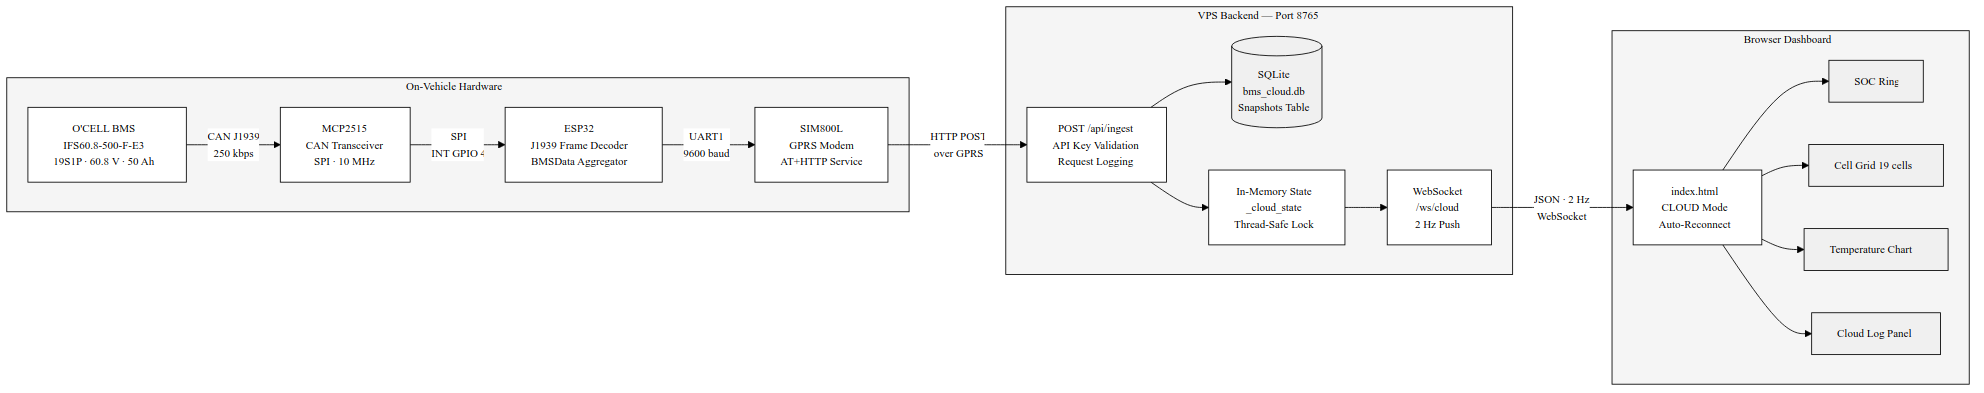
\includegraphics[width=0.92\textheight]{images/cloud-pipeline.png}%
    }
    \caption{Complete data pipeline from CAN bus to browser}
    \label{fig:cloud-pipeline}
\end{figure}

\subsubsection{Ingest Endpoint}

The \texttt{POST /api/ingest} endpoint is the sole entry point for ESP32 data. Its implementation:

\begin{enumerate}
    \item Validates the \texttt{X-Api-Key} header against the \texttt{BMS\_API\_KEY} environment variable. An incorrect key returns HTTP 401.
    \item Extracts the timestamp, device ID, cell count, SOC, and pack voltage from the JSON body for logging.
    \item Runs a non-blocking SQLite insert via \texttt{asyncio.run\_in\_executor()} to avoid blocking the event loop during disk I/O.
    \item Updates the in-memory \texttt{\_cloud\_state} dict atomically under a threading lock (because the serial reader thread and the asyncio event loop share this state).
    \item Appends a timestamped \texttt{[RECV]} entry to the cloud communication log.
    \item Returns \texttt{\{"status": "ok", "ts": ...\}} with HTTP 200.
\end{enumerate}

\subsubsection{SQLite Persistent Storage}

Received snapshots are persisted in a local SQLite database (\texttt{backend/bms\_cloud.db}) for historical analysis and post-session review. The schema is intentionally minimal:

\begin{verbatim}
CREATE TABLE IF NOT EXISTS snapshots (
    id        INTEGER PRIMARY KEY AUTOINCREMENT,
    ts        TEXT    NOT NULL,
    device_id TEXT    NOT NULL DEFAULT 'esp32',
    payload   TEXT    NOT NULL
);
\end{verbatim}

The full JSON payload is stored as a text column, which avoids schema migrations when new fields are added to the firmware. Queries for the \texttt{/api/history} endpoint retrieve records ordered by descending \texttt{id} (newest first) with a configurable limit. SQLite was chosen over a full database server because:

\begin{itemize}
    \item At one snapshot per 5 seconds, a full day of operation produces only $\sim$17,000 rows ($\sim$10 MB), well within SQLite's performance envelope.
    \item No separate database process or network socket is required.
    \item The database file can be copied directly from the VPS for offline analysis with standard tools.
\end{itemize}

A similar storage mechanism was also implemented on the Python emulator side, where generated telemetry records are stored locally in SQLite before being transmitted through a TCP socket client.

\subsubsection{In-Memory State and WebSocket Push}

In addition to SQLite, the server maintains an in-memory dictionary (\texttt{\_cloud\_state}) that always holds the most recently received snapshot. This allows the \texttt{/ws/cloud} WebSocket handler to serve browser clients at 2 Hz with zero disk I/O per push.

The in-memory state is initialized to \texttt{\{"connected": false, "source": "cloud"\}} on startup. The dashboard interprets \texttt{connected: false} as a "waiting for ESP32" state and displays a yellow indicator to the user rather than an error.

% ─────────────────────────────────────────────────────────────────────────────
\subsection{Remote Monitoring Dashboard}

\subsubsection{Architecture}

The dashboard is a \textbf{single-page web application} served as a static HTML file (\texttt{frontend/index.html}) directly by the FastAPI backend via \texttt{GET /}. No separate web server, build tool, or JavaScript framework is required. All rendering logic is contained in vanilla JavaScript.

The dashboard connects to the backend over \textbf{WebSocket}, which provides a persistent, low-latency bidirectional channel. In SERIAL mode the WebSocket endpoint is \texttt{/ws} (10 Hz push from the serial reader); in CLOUD mode it is \texttt{/ws/cloud} (2 Hz push from the in-memory state). The user switches between modes using a toggle button in the header.

\subsubsection{Dashboard Panels}

Table~\ref{tab:cloud-dashboard-panels} summarizes the information panels displayed by the dashboard.

\begin{table}[h]
    \centering
    \caption{Dashboard Panel Summary}
    \label{tab:cloud-dashboard-panels}
    \begin{tabular}{lp{9cm}}
        \toprule
        \textbf{Panel} & \textbf{Contents} \\
        \midrule
        SOC ring        & Animated circular gauge showing voltage-derived SOC (\texttt{battery.soc}). BMS coulomb-counter SOC (\texttt{battery.soc\_bms}) is displayed below. \\
        Pack KPIs       & Pack voltage, current, discharge limit, charge request, and cell count in a card grid. \\
        Cell grid       & All 19 cells — individual voltage bars color-coded by threshold (overvoltage / full / good / normal / low / undervoltage), with min/max/avg/spread statistics. \\
        Temperature     & Up to 4 temperature probe readings with color-coded bars and a rolling time-series chart. \\
        Serial monitor  & Raw CAN frame log with text export and Excel export capabilities. \\
        Cloud log       & Real-time cloud communication events (RECV / WS / ERR), polled from \texttt{/api/cloud-log} every 2 seconds, independent of the SERIAL/CLOUD source toggle. \\
        \bottomrule
    \end{tabular}
\end{table}

\subsubsection{Connection Status Indicator}

The dashboard header contains a three-state connection indicator that provides immediate visual feedback:

\begin{description}
    \item[\textcolor{green}{Green — Live}] WebSocket is open and the last received message contained \texttt{connected: true}.
    \item[\textcolor{yellow}{Yellow — Waiting}] WebSocket is open but \texttt{connected: false} (backend is running but no ESP32 data has arrived yet).
    \item[\textcolor{red}{Red — Disconnected}] WebSocket is closed or encountered a network error.
\end{description}

\subsubsection{Auto-Reconnect}

If the WebSocket closes unexpectedly (server restart, network interruption), the browser automatically attempts to reconnect every 5 seconds. The overlay is re-displayed during the disconnected interval. This behavior is handled entirely client-side and requires no intervention from the user.

% ─────────────────────────────────────────────────────────────────────────────
\subsection{Security \& Cybersecurity}

\subsubsection{API Key Authentication}

The \texttt{POST /api/ingest} endpoint is protected by a shared secret transmitted as the \texttt{X-Api-Key} HTTP header. The server compares the received key against the \texttt{BMS\_API\_KEY} environment variable. Requests with a missing or incorrect key are rejected with HTTP 401 before any data is read from the body, and an \texttt{[ERR]} entry is appended to the cloud log.

The API key is configured separately on the firmware (\texttt{VPS\_API\_KEY} in \texttt{include/secrets.h}, which is in \texttt{.gitignore}) and on the server (environment variable), so the secret is never committed to the repository.

\subsubsection{Transport Layer}

Communication between the SIM800L and the VPS uses plain HTTP. While this means the payload is not encrypted in transit, the following mitigating factors apply to this deployment context:

\begin{itemize}
    \item The data transmitted is battery telemetry (voltages, temperatures, SOC) — not personally identifiable information or control commands.
    \item The VPS port is firewalled to accept connections only on the designated port.
    \item The API key protects against unauthorized data injection.
\end{itemize}

For a production deployment, upgrading to HTTPS requires enabling TLS on the SIM800L (\texttt{AT+HTTPSSL=1}) and deploying a self-signed or CA-signed certificate, or using an Nginx reverse proxy with Let's Encrypt on the VPS side.

\subsubsection{WebSocket and Dashboard Access}

The dashboard itself is served over plain HTTP and the WebSocket connection is unencrypted. Since the dashboard is intended for use on a private network or VPN-protected VPS, this is considered acceptable for the current project scope. Adding HTTPS would require an SSL certificate (e.g., from Let's Encrypt) and an Nginx reverse proxy, which is a straightforward extension if needed.

% ─────────────────────────────────────────────────────────────────────────────
\subsection{API Documentation}

The FastAPI backend exposes the following endpoints, summarized in Table~\ref{tab:api-endpoints}. FastAPI generates interactive Swagger UI documentation automatically at \texttt{/docs} when the server is running.

\begin{table}[h]
    \centering
    \caption{Backend API Endpoint Reference}
    \label{tab:api-endpoints}
    \begin{tabular}{llp{7.5cm}}
        \toprule
        \textbf{Method} & \textbf{Path} & \textbf{Description} \\
        \midrule
        GET  & \texttt{/}                        & Serves the dashboard HTML file. \\
        WS   & \texttt{/ws}                      & Serial stream — pushes BMS JSON to the browser at 10 Hz. Active when an ESP32 is connected via USB. \\
        WS   & \texttt{/ws/cloud}                & Cloud stream — pushes the latest in-memory snapshot at 2 Hz. \\
        POST & \texttt{/api/ingest}              & Receives a BMS JSON snapshot from the ESP32. Requires header \texttt{X-Api-Key}. Returns \texttt{\{status: ok, ts: ...\}}. \\
        GET  & \texttt{/api/latest}              & Returns the most recent snapshot as JSON. \\
        GET  & \texttt{/api/history?limit=N}     & Returns the last $N$ snapshots from SQLite, newest first (default $N$ = 100, max 1000). \\
        GET  & \texttt{/api/cloud-log}           & Returns the last 100 cloud communication events as a JSON array of timestamped strings. \\
        \bottomrule
    \end{tabular}
\end{table}

\subsubsection{Ingest Payload Schema}

The JSON body sent by the ESP32 to \texttt{POST /api/ingest} uses a \textbf{nested object structure} organized into five top-level sections. This design allows each subsystem (battery, thermal, solar, DC/DC, vehicle) to be extended independently without changing the ingest endpoint. Table~\ref{tab:json-schema-top} describes the top-level envelope, and Table~\ref{tab:json-schema-battery} expands the \texttt{battery} object.

\begin{table}[h]
    \centering
    \caption{ESP32 JSON Payload — Top-Level Envelope}
    \label{tab:json-schema-top}
    \begin{tabular}{lll}
        \toprule
        \textbf{Field} & \textbf{Type} & \textbf{Description} \\
        \midrule
        \texttt{device\_id}   & string & Configurable in \texttt{secrets.h} \\
        \texttt{timestamp}    & string & Network time from \texttt{AT+CCLK?} (or \texttt{uptime\_ms} fallback) \\
        \texttt{source}       & string & Always \texttt{"esp32-SIM800L"} \\
        \texttt{connected}    & bool   & Always \texttt{true} when sent by the ESP32 \\
        \texttt{frame\_count} & int    & Cumulative CAN frames decoded since boot \\
        \texttt{fault\_level} & int    & 0 = normal, 1 = serious fault \\
        \texttt{error\_code}  & int    & BMS fault code (see Table~\ref{tab:fault-codes}) \\
        \texttt{battery}      & object & Battery pack data — see Table~\ref{tab:json-schema-battery} \\
        \texttt{temperatures} & object & Thermal data from all probes \\
        \texttt{solar}        & object & Solar MPPT data (pre/post converter) \\
        \texttt{dc\_dc}       & object & DC/DC converter outputs (64 V and 12 V rails) \\
        \texttt{vehicle}      & object & Vehicle-level status (handbrake, etc.) \\
        \bottomrule
    \end{tabular}
\end{table}

\begin{table}[h]
    \centering
    \caption{ESP32 JSON Payload — \texttt{battery} Object Fields}
    \label{tab:json-schema-battery}
    \begin{tabular}{lll}
        \toprule
        \textbf{Field} & \textbf{Type} & \textbf{Description} \\
        \midrule
        \texttt{pack\_v}          & float  & Pack voltage [V], 0.1 V resolution \\
        \texttt{pack\_current\_a} & float  & Pack current [A], + = discharge, $-$ = charge \\
        \texttt{soc}              & float  & Voltage-derived SOC [\%] \\
        \texttt{soc\_bms}         & int    & BMS coulomb-counter SOC [\%] \\
        \texttt{max\_disch\_a}    & float  & Maximum discharge current limit [A] \\
        \texttt{cell\_count}      & int    & Number of active cells decoded \\
        \texttt{cell\_avg\_mv}    & int    & Average cell voltage [mV] \\
        \texttt{cell\_min\_mv}    & int    & Minimum cell voltage [mV] \\
        \texttt{cell\_max\_mv}    & int    & Maximum cell voltage [mV] \\
        \texttt{cell\_spread\_mv} & int    & Max $-$ min cell voltage [mV] \\
        \texttt{cells}            & array  & 1-based array of \texttt{\{"mv", "status"\}} objects; index 0 = \texttt{null} \\
        \texttt{charger}          & object & \texttt{max\_charge\_v}, \texttt{max\_charge\_a}, \texttt{start\_signal} \\
        \texttt{status}           & object & Bit-field flags: charging, discharging, ready, contactors \\
        \bottomrule
    \end{tabular}
\end{table}

The \texttt{temperatures} object contains \texttt{battery\_avg\_c}, \texttt{battery\_min\_c}, \texttt{battery\_max\_c}, and a 1-based \texttt{battery\_cells} array (index 0 = \texttt{null}, indices 1--4 = probe readings in \textdegree C). Fields for sensors not yet instrumented (\texttt{motor\_c}, \texttt{mppt\_c}, \texttt{cabin\_c}) are present with value \texttt{null}, enabling the dashboard to display placeholders without schema changes when those sensors are added. The same pattern applies to \texttt{solar} and \texttt{dc\_dc} sub-objects.

\subsubsection{Example API Interaction}

The following \texttt{curl} command simulates an ESP32 posting a snapshot to the server during testing. On a successful ingest the server returns a timestamped acknowledgement and pushes the payload to any browser connected to \texttt{/ws/cloud} within 2 seconds.

\begin{verbatim}
curl -X POST http://YOUR_VPS_IP:8787/api/ingest \
  -H "Content-Type: application/json"           \
  -H "X-Api-Key: bako-bms-2024"                \
  -d '{
    "device_id": "esp32-bms-001",
    "connected": true,
    "fault_level": 0,
    "battery": {
      "soc": 87.4, "pack_v": 62.3,
      "cell_count": 19,
      "cells": [null, {"mv": 3280, "status": "good"}]
    },
    "temperatures": { "battery_avg_c": 21.0,
                      "battery_cells": [null, 21.0, 22.0, null, null] }
  }'
\end{verbatim}

\noindent The server responds with \texttt{\{"status": "ok", "ts": "2026-04-18T09:32:11.123456"\}}.
